\documentclass[runningheads,a4paper]{llncs}

\usepackage[american]{babel}

%better font, similar to the default springer font
%cfr-lm is preferred over lmodern. Reasoning at http://tex.stackexchange.com/a/247543/9075
\usepackage[%
rm={oldstyle=false,proportional=true},%
sf={oldstyle=false,proportional=true},%
tt={oldstyle=false,proportional=true,variable=true},%
qt=false%
]{cfr-lm}
%
%if more space is needed, exchange cfr-lm by mathptmx
%\usepackage{mathptmx}

\usepackage{graphicx}

%extended enumerate, such as \begin{compactenum}
\usepackage{paralist}

%put figures inside a text
%\usepackage{picins}
%use
%\piccaptioninside
%\piccaption{...}
%\parpic[r]{\includegraphics ...}
%Text...

%Sorts the citations in the brackets
%\usepackage{cite}

%for easy quotations: \enquote{text}
\usepackage{csquotes}

\usepackage[T1]{fontenc}

%enable margin kerning
\usepackage{microtype}

%for demonstration purposes only
\usepackage[math]{blindtext}

%tweak \url{...}
\usepackage{url}
%nicer // - solution by http://tex.stackexchange.com/a/98470/9075
\makeatletter
\def\Url@twoslashes{\mathchar`\/\@ifnextchar/{\kern-.2em}{}}
\g@addto@macro\UrlSpecials{\do\/{\Url@twoslashes}}
\makeatother
\urlstyle{same}
%improve wrapping of URLs - hint by http://tex.stackexchange.com/a/10419/9075
\makeatletter
\g@addto@macro{\UrlBreaks}{\UrlOrds}
\makeatother

%diagonal lines in a table - http://tex.stackexchange.com/questions/17745/diagonal-lines-in-table-cell
%slashbox is not available in texlive (due to licensing) and also gives bad results. This, we use diagbox
%\usepackage{diagbox}

%required for pdfcomment later
\usepackage{xcolor}

% new packages BEFORE hyperref
% See also http://tex.stackexchange.com/questions/1863/which-packages-should-be-loaded-after-hyperref-instead-of-before

%enable hyperref without colors and without bookmarks
\usepackage[
%pdfauthor={},
%pdfsubject={},
%pdftitle={},
%pdfkeywords={},
bookmarks=false,
breaklinks=true,
colorlinks=true,
linkcolor=black,
citecolor=black,
urlcolor=black,
%pdfstartpage=19,
pdfpagelayout=SinglePage,
pdfstartview=Fit
]{hyperref}
%enables correct jumping to figures when referencing
\usepackage[all]{hypcap}

%enable nice comments
\usepackage{pdfcomment}
\newcommand{\commentontext}[2]{\colorbox{yellow!60}{#1}\pdfcomment[color={0.234 0.867 0.211},hoffset=-6pt,voffset=10pt,opacity=0.5]{#2}}
\newcommand{\commentatside}[1]{\pdfcomment[color={0.045 0.278 0.643},icon=Note]{#1}}

%compatibality with TODO package
\newcommand{\todo}[1]{\commentatside{#1}}

%enable \cref{...} and \Cref{...} instead of \ref: Type of reference included in the link
\usepackage[capitalise,nameinlink]{cleveref}
%Nice formats for \cref
\crefname{section}{Sect.}{Sect.}
\Crefname{section}{Section}{Sections}
\crefname{figure}{Fig.}{Fig.}
\Crefname{figure}{Figure}{Figures}

\usepackage{xspace}
%\newcommand{\eg}{e.\,g.\xspace}
%\newcommand{\ie}{i.\,e.\xspace}
\newcommand{\eg}{e.\,g.,\ }
\newcommand{\ie}{i.\,e.,\ }

%introduce \powerset - hint by http://matheplanet.com/matheplanet/nuke/html/viewtopic.php?topic=136492&post_id=997377
\DeclareFontFamily{U}{MnSymbolC}{}
\DeclareSymbolFont{MnSyC}{U}{MnSymbolC}{m}{n}
\DeclareFontShape{U}{MnSymbolC}{m}{n}{
    <-6>  MnSymbolC5
   <6-7>  MnSymbolC6
   <7-8>  MnSymbolC7
   <8-9>  MnSymbolC8
   <9-10> MnSymbolC9
  <10-12> MnSymbolC10
  <12->   MnSymbolC12%
}{}
\DeclareMathSymbol{\powerset}{\mathord}{MnSyC}{180}

% correct bad hyphenation here
\hyphenation{op-tical net-works semi-conduc-tor}

\begin{document}

%Works on MiKTeX only
%hint by http://goemonx.blogspot.de/2012/01/pdflatex-ligaturen-und-copynpaste.html
%also http://tex.stackexchange.com/questions/4397/make-ligatures-in-linux-libertine-copyable-and-searchable
%This allows a copy'n'paste of the text from the paper
\input glyphtounicode.tex
\pdfgentounicode=1

\title{ECE 657A Project Report}
%If Title is too long, use \titlerunning
%\titlerunning{Short Title}

%Single insitute
\author{Laura McCrackin (20262085),  Tianhui Huang (20587328) \and Yuzhou Wang (20609396)}
%If there are too many authors, use \authorrunning
%\authorrunning{First Author et al.}
\institute{University of Waterloo}

%Multiple insitutes
%Currently disabled
%
\iffalse
%Multiple institutes are typeset as follows:
%\author{Firstname Lastname\inst{1} \and Firstname Lastname\inst{2} }
%If there are too many authors, use \authorrunning
%\authorrunning{First Author et al.}

\institute{
University of Waterloo\\
\email{...}\and
University of Waterloo\\
\email{...}
}
\fi
			
\maketitle
%%%%%%%%%%%%%   abstract need to be added!!!! %%%%%%%%%
\begin{abstract}
Traditionally, there are several methods to sovle the question answering problem. In our project, we are aiming to solve this problem by nueral network in attentive model.
\keywords{Deep Learning, Nueral Network, NLP}
\end{abstract}



%%%%%%%%%%%%%%%%%%%%%%%%%%%%%%%%%%%%%%%%%%%%%%%%%%%%%%%%%%%%%%%%%%%%%%%%%%%%%%%
\section{Introduction}\label{sec:intro}
%%%%%%%%%%%%%%%%%%%%%%%%%%%%%%%%%%%%%%%%%%%%%%%%%%%%%%%%%%%%%%%%%%%%%%%%%%%%%%%
%\blindtext\todo{Refine me}

%Winery~\cite{Winery} is graphical \commentontext{modeling}{modeling with one \enquote{l}, because of AE} tool.


Natural Language Processing (NLP), as one of the artificial intelligence topic, is becoming more and more popular recently. It can also be divided into several parts like text to speech, speech recognition, information retrieval, etc. Our project focuses on getting the information from a passage of text aiming to training machine to Read and Comprehend. When an article is given, the machine could automatically answer the questions. This project is one of the topic in Nature language processing, enabling computers to derive meaning from human or natural language input.  


\section{Dataset}
We used the Machine Comprehension Test (MCTest) dataset created by Microsoft [1]. The authors of stories are all workers, residing in the United States. The average worker is 36 years old, more educated than the United States population in general, and the majority of workers are female. Workers were instructed to write a short fictional story, and to write as if for a child in grade school. Workers were also asked to provide four reading comprehension questions pertaining to their story and, for each, four multiple-choice answers. Workers were requested to provide 'reasonable' incorrect answers that at least include words from the story so that their solution is not trivial. Finally, workers were asked to design their questions and answers such that at least two of the four questions required multiple sentences from the story to answer them. That is, for those questions it should not be possible to find the answer in any individual sentence. 
The MCTest corpus contains two sets of stories, named MC160 and MC500, and containing 160 and 500 stories respectively. MC160 was gathered first, then some improvements were made before gathering MC500. Adding a Grammar Test to form the MC500. 
In addition to the details described above, MC160 workers were given a target elementary grade school level (1-4) and a sample story matching that grade level5. 
For the story generate, they ensured that the data is the same quality as another set and also limited the text to children stories, so that it could be easily understand.The  vocabulary is also limited: the lowercase words in the story, questions, and answers were stemmed from list of approximately 8000 words that a 7 year old is likely to know. Multiple-sentence questions: At least two of the questions need multiple sentences to answer. As each story is fictional, the answers can only be found in the story itself, which requires high-level machine comprehension without any world knowledge.


\section{Review of literature}
Traditional baseline methods:majority baseline (maximum frequency) picks the entity most frequently observed in the context document.
Exclusive majority (exclusive frequency) chooses the entity most frequently observed in the context but not observed in the query. The idea behind this exclusion is that the placeholder is unlikely to be mentioned twice in a single Cloze form query[2]. 
Word Distance Benchmark: The main idea is that choose the shortest distance among all of the answers to the question key words.


There are also several traditinal methods.Firstly, it is traditional Frame-Semantic Parsing. Frame-semantic parsing attempts to identify predicates and their arguments, allowing models access to information about 'who did what to whom'. And we could see some of the language strategy patterns as figure 1.

\begin{figure}[p]
	\centering
	\begin{subfigure}{.5\textwidth}
		\centering
		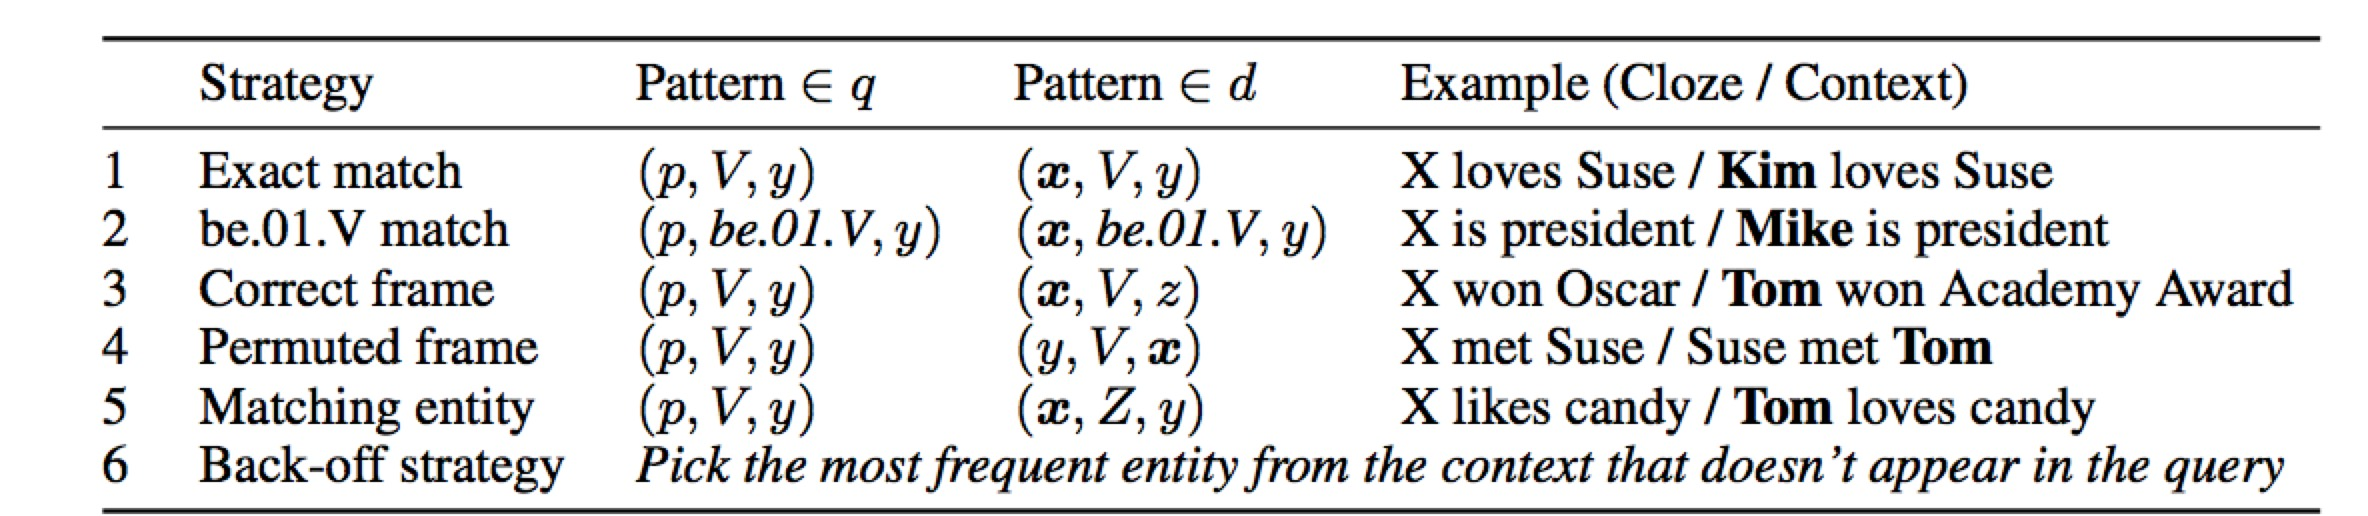
\includegraphics[width=1\linewidth]{../pic/parsing.png}
		
		\label{figure 1:Frame-Semantic Parsing}
	\end{subfigure}	
\end{figure}




%\begin{figure}[p]
%	\centering
%	\begin{subfigure}{.5\textwidth}
%		\centering
%		\includegraphics[width=1\linewidth]{../images-update/1-(3)-2.png}
%		\caption{ROC}
%		\label{fig:sub1}
%	\end{subfigure}
	
%\end{figure}



But this method has some limitations for can not possess the capability to generalize through a language model beyond exploiting one during the parsing phase[2]. And what is more, teaching machines to read natural language documents remains an elusive challenge. Machine reading systems can be tested on their ability to answer questions posed on the contents of documents that they have seen, but until now large scale training and test datasets have been missing for this type of evaluation. In other words, those are limited on training dataset.

Other people also have the idea of comprehension with Syntax, Frames, and Semantics method.Semantic: frame semantic parsing is aimed to extract frame-specific predicate-argument structures from sentences[3].
Syntax: given each candidate answer, we attempt to transform the question to a statement using the extraction rules[4]. We could see figure 2 for sematic and figure 3 for syntax.
%\begin{figure}[p]
%	\centering
%	\begin{subfigure}{.5\textwidth}
%		\centering
%		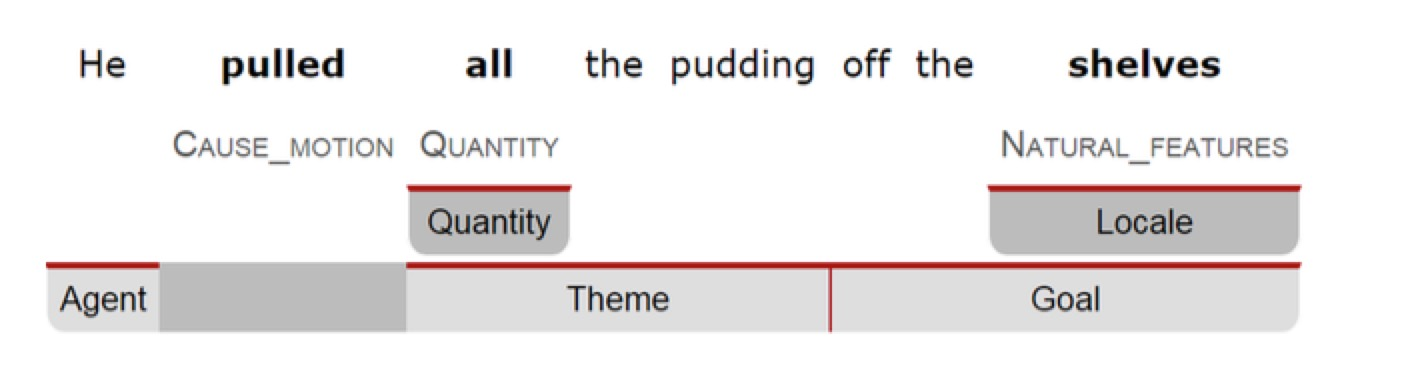
\includegraphics[width=1\linewidth]{../pic/sematic.png}
%		\caption{ROC}
%		\label{figure 2:sematic parsing}
%	\end{subfigure}
	
%\end{figure}

%\begin{figure}[p]
%	\centering
%	\begin{subfigure}{.5\textwidth}
%		\centering
%		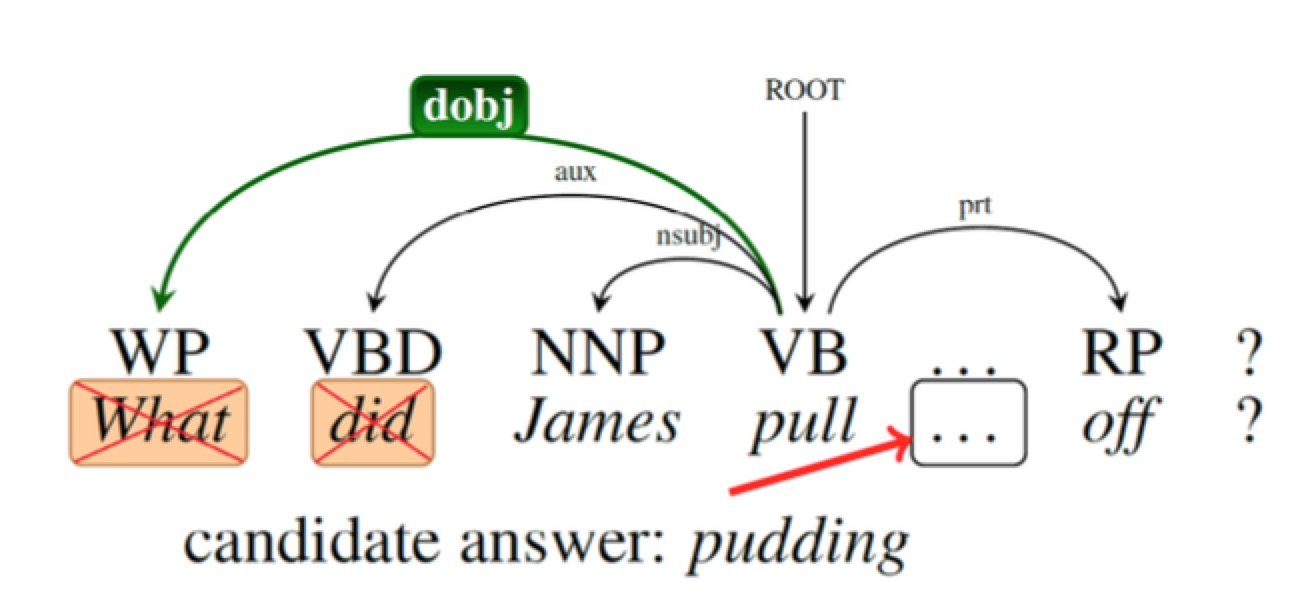
\includegraphics[width=1\linewidth]{../pic/syntax.png}
%		\caption{ROC}
%		\label{figure 3:syntax}
%	\end{subfigure}	
%\end{figure}

But according to the error analysis suggests that deeper linguistic analysis and inferential reasoning can yield further improvements on this task.


Comprehension with Discourse Relations[5].The model jointly identifies relevant sentences, establishes relations between them and predicts an answer. The key idea is to implant discourse analysis into a joint model for comprehension. As we could see in picture 4.And the drawback of this model is that the accuracy varies significantly according to the question type. Which means not really stable. 
%\begin{figure}[p]
%	\centering
%	\begin{subfigure}{.5\textwidth}
%		\centering
%		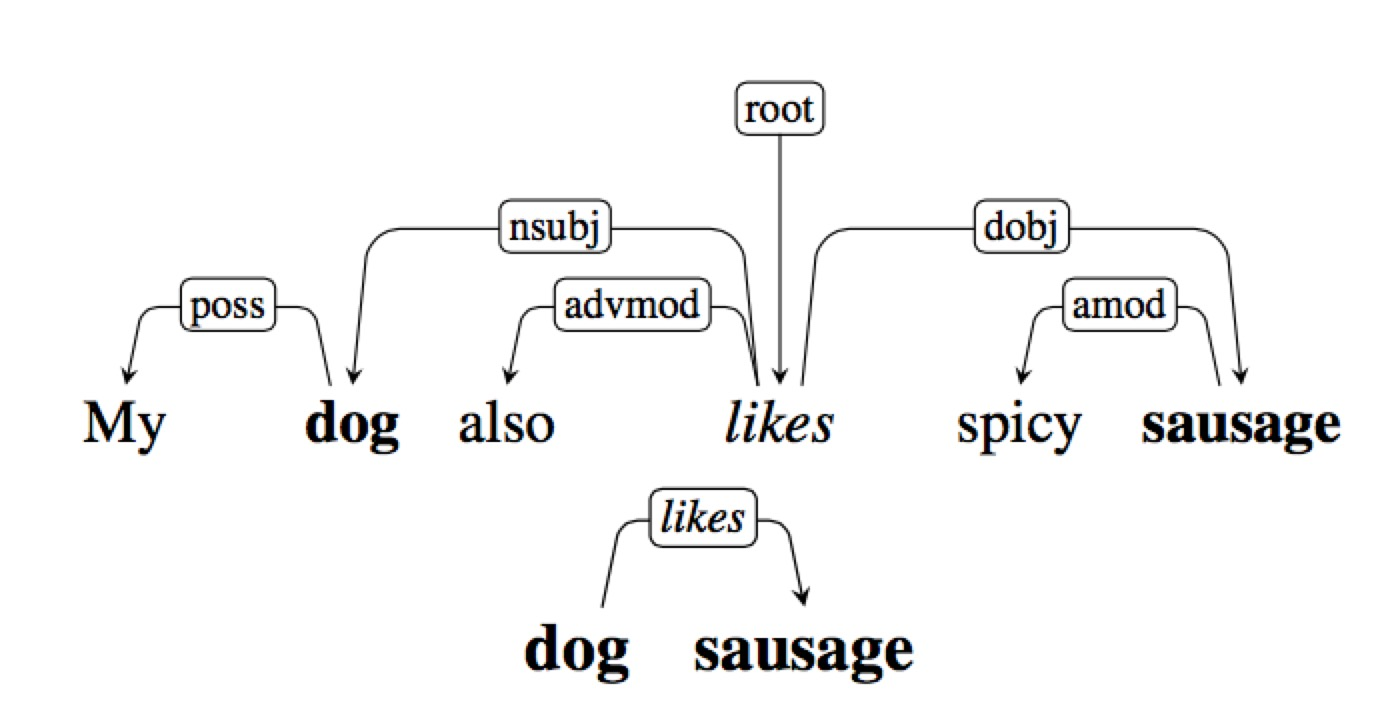
\includegraphics[width=1\linewidth]{../pic/disclosure.png}
%		\caption{ROC}
%		\label{figure 4:disclosure method}
%	\end{subfigure}
%\end{figure}

Comprehension for Learning Answer-Entailing Structures[6].We posit that there is a hidden (latent) structure that explains the relation between the question, correct answer, and text. For this given structure, the correctness of the answer is evident. Since the structure is latent, it must be inferred. Firstly, we should presents a unified max-margin framework that learns to find these hidden structures (given a corpus of question-answer pairs), and then uses what it learns to answer machine comprehension questions on novel texts. We could see this from figure 5. But the drawback of this method is that since inference is cheaply modelled via alignment structure, we lack the ability to deeply reason about facts or numbers. 
%\begin{figure}[p]
%	\centering
%	\begin{subfigure}{.5\textwidth}
%		\centering
%		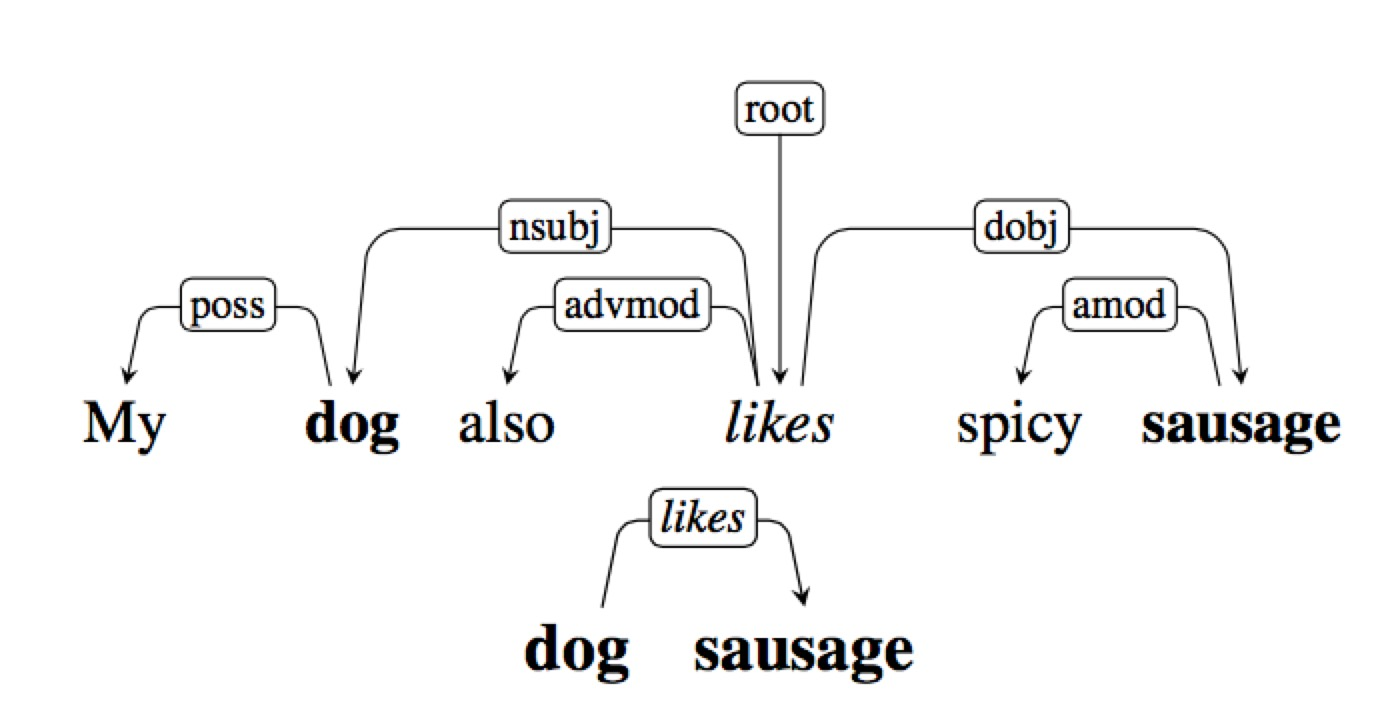
\includegraphics[width=1\linewidth]{../pic/disclosure.png}
%		\caption{ROC}
%		\label{figure 5:answer entailing method}
%	\end{subfigure}
%\end{figure}


\section{Research for Neural Network}
Firstly, some basic concept for RNN and ANN.In machine learning and cognitive science, artificial neural networks (ANNs) are a family of models inspired by biological neural networks (the central nervous systems of animals, in particular the brain) and are used to estimate or approximate functions that can depend on a large number of inputs and are generally unknown. Artificial neural networks are generally presented as systems of interconnected 'neurons' which exchange messages between each other. 
An ANN is typically defined by three types of parameters:
The interconnection pattern between the different layers of neurons
The learning process for updating the weights of the interconnections
The activation function that converts a neuron's weighted input to its output activation.
Contrary to feedforward networks, recurrent neural networks (RNNs) are models with bi-directional data flow. While a feedforward network propagates data linearly from input to output, RNNs also propagate data from later processing stages to earlier stages. RNNs can be used as general sequence processors.
For RNN model, there are several types, like Fully recurrent network, Hopfield network, Elman networks and Jordan networks, Echo state network and Long short term memory network,etc.

The Long short term memory (LSTM) network, developed by Hochreiter and Schmidhuber in 1997[7] is an artificial neural network structure that unlike traditional RNNs doesn't have the vanishing gradient problem (compare the section on training algorithms below). It works even when there are long delays, and it can handle signals that have a mix of low and high frequency components. LSTM RNN outperformed other methods in numerous applications such as language learning[8] and connected handwriting recognition[9].



The Deep LSTM Reader embed long sequences into a vector representation which contains enough information to generate a full translation in another language. The result is that this model processes each document query pair as a single long sequence. Given the embedded document and query the network predicts which token in the document answers the query. So this one is the old version of neural networking. We could see from figure 6 for LSTM.

%\begin{figure}[p]
%	\centering
%	\begin{subfigure}{.5\textwidth}
%		\centering
%		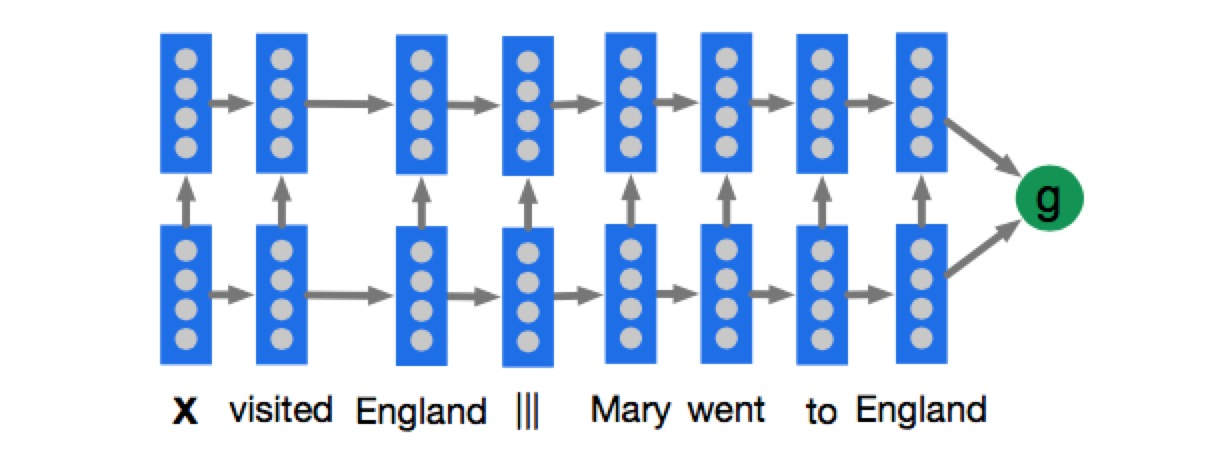
\includegraphics[width=1\linewidth]{../pic/LSTM.png}
%		\caption{ROC}
%		\label{figure 6:LSTM}
%	\end{subfigure}
%\end{figure}



The Impatient Reader focuses on the passages of a context document that are most likely to inform the answer to the query. We can go further by equipping the model with the ability to reread from the document as each query token is read. The result is an attention mechanism that allows the model to recurrently accumulate information from the document as it sees each query token, ultimately outputting a final joint document query representation for the answer prediction. We could see figure 7 for impatient reader.
%\begin{figure}[p]
%	\begin{subfigure}{.5\textwidth}
%		\centering
%		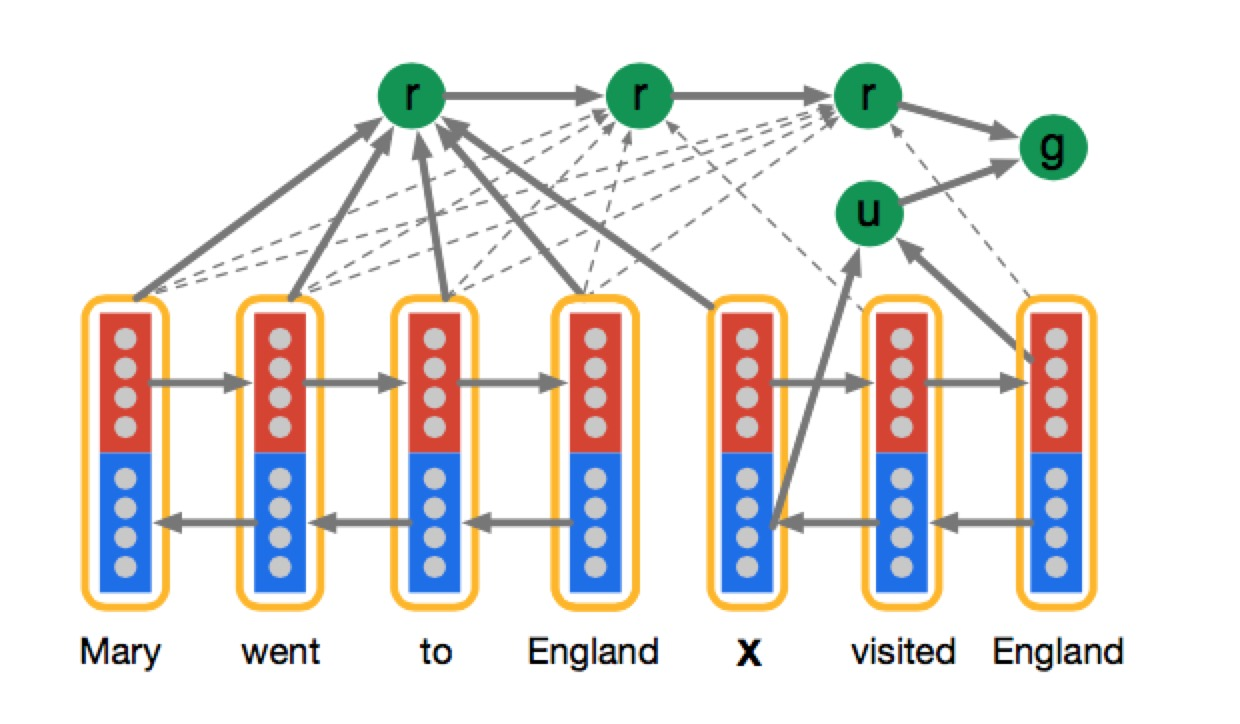
\includegraphics[width=1\linewidth]{../pic/impa.png}
%		\caption{ROC}
%		\label{figure 7:impatient reader}
%	\end{subfigure}
%\end{figure}

The Attentive Reader can be viewed as a generalization of the application of Memory Networks to question answering. That model employs an attention mechanism at the sentence level where each sentence is represented by a bag of embeddings. This model could fix the bottleneck for the width of different words. This attention model first encodes the document and the query using separate bidirectional single layer LSTMs. This task has been tricky because of the number of parameters that must be fine-tuned.
Although this method cannot be backwards checking as impatient reader but according to some article, these two methods have the similar results, so our group used this model. We could see figure 8 for attentive model.
%\begin{figure}[p]
%	\centering
%	\begin{subfigure}{.5\textwidth}
%		\centering
%		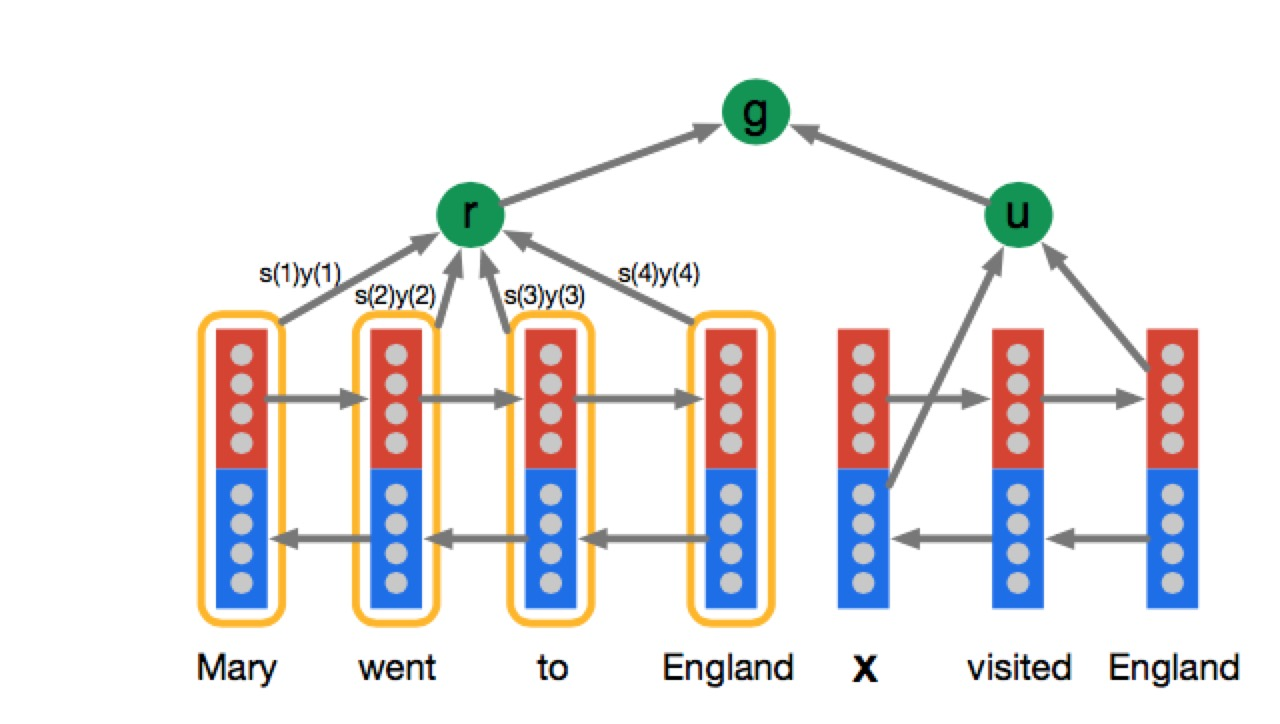
\includegraphics[width=1\linewidth]{../pic/attentive.png}
%		\caption{ROC}
%		\label{figure 8:attentive model}
%	\end{subfigure}	
%\end{figure}

\section{Description of the project task and the used methods}
For data preprocessing, we use python NLTK library.
For deep learning part, we use blocks and fuels, Theano framework for deep learning part. 
Blocks and fuel[10] are two Python frameworks to train neural networks on large datasets. Blocks is based on Theano, a linear algebra compiler with CUDA-support. It facilitates the training of complex neural network models by providing parametrized Theano operations, attaching metadata to Theano symbolic computational graph, and providing an extensive set of utilities to assist training the networks, e.g. training algorithms, logging, monitoring, visualization, and serialization. Fuel provides a standard format for machine learning datasets. It allows the user to easily iterate over large datasets, performing many types of pre-processing on the fly[10].
Blocks and Fuel are being developed by the Montreal Institute of Learning Algorithms (MILA) at the University of Montreal. Their focus lies on quick prototyping of complex neural network models. 
Instead of introducing new abstract objects representing 'models' or 'layers'. Blocks annotates the theano computational graph, maintaining the flexibility of theano while making large models manageable. 
Data processing is an integral part of training neural networks, which is not addressed by many of the aforementioned frameworks. Fuel aims to fill this gap. It provides tools to download datasets and iterate/preprocess them efficiently. 

Theano is a popular choice for the implementation of neural networks. Blocks and many other libraries, such as Pylearn2, build on Theano by providing reusable components that are common in neural networks, such as linear transformations followed by non-linear activations, or more complicated components such as LSTM units. In Blocks these components are referred to as 'bricks' or 'parametrized Theano operations'. 
Blocks comes with a large number of 'bricks'. 
The gradient descent training algorithm in Blocks is composed of different 'step rules' that modify the descent direction (learning rate scaling, momentum, gradient clipping, weight norm clipping, etc.). A variety of algorithms such as AdaGrad, ADADELTA, Adam, RMSProp are available as step rules. But in our project, we use gradient descent algorithm.
The goal of fuel is to provide a common interface to a variety of data formats and published datasets such as MNIST, CIFAR-10, ImageNet, etc. while making it easy for users to write an interface to new datasets. 
Blocks relies on Fuel for its data interface, but Fuel can easily be used by other machine learning frameworks that interface with datasets. 
Fuel offers built-in scripts that automate the task of downloading datasets, (similar to e.g. skdata1) and converting them to Fuel HDF5 specification. 
The fuel download script is used to download raw data files. Downloading the raw MNIST data files is as easy as typing fuel download mnist. The fuel convert script is used to convert raw data files into HDF5-format. 
Reproducibility being an important feature of both Fuel and Blocks, the fuel convert script automatically tags all files it creates with relevant module and interface versions and the exact command that was used to generate these files. Inspection of this metadata is done with the fuel info script. 
Theano is a compiler for mathematical expressions in Python that combines the convenience of NumPy syntax with the speed of optimized native machine language. The user composes mathematical expressions in a high-level description that mimics NumPy syntax and semantics, while being statically typed and functional (as opposed to imperative). These expressions allow Theano to provide symbolic differentiation[11].
Theano was introduced to the machine learning community as a CPU and GPU mathematical compiler, demonstrating how it can be used to symbolically define mathematical functions, automatically derive gradient expressions, and compile these expressions into executable functions that outperform implementations using other existing tools[12].
\section{compare of original method and the method we used}
For preprocessing part:
1) split the story dataset into one story one file, and do the same thing on the related answer dataset 
2) label correct answers obtained from corresponding answer file
in each story file 
3) convert abbreviation using Regular Expression and numbers to words using a recrusive function implemented by ourselves on story, questions and answers in each story file 
4) lowercase all text of stories, tokenize them, then build a vocabulary file without repeat words
5) find out entities in each story and replace them with entity identifiers, then add the corresponding entity and entity identifier list below the questions
6) delete punctuations on the text of each story, the reason for doing this after step 5 is that punctuations will help to identify the entities 
7) remove stop words, lemmatization and stemming on each story dealing with NLTK library functions
8) preprocess both questions and answers using the entity list gained from step 5

The Attentive Reader can be viewed as a generalisation of the application of Memory Networks to question answering. That model employs an attention mechanism at the sentence level where each sentence is represented by a bag of embeddings. The Attentive Reader employs a finer grained token level attention mechanism where the tokens are embedded given their entire future and past context in the input document. 
The representation r of the document d is formed by a weighted sum of these output vectors. These weights are interpreted as the degree to which the network attends to a particular token in the document. Given this attention score the embedding of the document r is computed as the weighted sum of the token embeddings. 

According to a recent google paper, for the Deep LSTM Reader, they consider hidden layer sizes [64, 128, 256], depths [1, 2, 4], initial learning rates [1E3, 5E4, 1E4, 5E5], batch sizes [16, 32] and dropout [0.0, 0.1, 0.2]. Evaluated two types of feeds. In the cqa setup they feed first the context document and subsequently the question into the encoder, while the qca model starts by feeding in the question followed by the context document. For the attention models they consider hidden layer sizes [64, 128, 256], single layer, initial learning rates [1E4, 5E5, 2.5E5, 1E5], batch sizes [8, 16, 32] and dropout [0, 0.1, 0.2, 0.5]. For all models we used asynchronous RmsProp [20] with a momentum of 0.9 and a decay of 0.95. 


For deep mind model output, we define function 1,for a given document(d) and query(q), we could estimate the probability of word a being the correct answer.We define a new method to determine which possible answer is the correct one. As we could see from function 2, that is, the correct answer should be the most similar to the most highly attended words in the story. We use the similarity metric, as we could see from function 3. For a multiple choice answer of length n words. Take the weighted average of the attention each word from the multiple choice answer has within the story. If a word in the answer is not in the story, we then chooce to use word distance from the closest attended word as apenalty.\newline
Function 1: \newline
 here some error for the function
%p(a|d,q) \propto exp (W(a) g(d,q)), a \epsilon V
W stands for weight, g stands for vector embedding and v stands for vocabulary \newline
Function 2: \newline
C=max[S(Ci,p(a|d,q))] \newline
here C is for correct choice, S is for similarity, Ci is for ith multiple choice answer, i from 1 to 4.
\newline
Function 3:\newline
%S(Ci,p(a|d,q))=\sum_{j=1}^{n} p(aj|d,q)/n    
here still a small problem and did not figure out yet
%S(Ci,p(a|d,q))=\sigma p(aj|d,q)/n
%%%%%%%
\section{run time}
As for the run time, and computational complexity. Original Attentive Reader: trained for 2-4 days using two NVIDIA Titan Black GPUs (PassMark score 8,667 each)
Our setup: one NVIDIA GTX 660 GPU  inside older machine: Core 2 Quad Q8300, 8GB DDR2 PC6400 RAM. And the training time is around one day.
For result, we first calculate weight matrix multiply vector embedding matrix for each word, and choose the highest possibility. The higher the possibility it is, the more colorful the words could be.



\section{Implementation details and experimental setup}
For preprocessing part, we firstly setup the NLTK working environment with python and later import some libraries like stem, tokenize, corpus, etc. We deal with deleting punctuation like ',' '.',etc. Later we also extract questions pattern like 'when', 'how', etc. we change numbers into English words by dictionary. We also do the following step for text preprocessing. 

1) split the story dataset into one story one file, and do the same thing on the related answer dataset 
2) label correct answers obtained from corresponding answer file
in each story file 
3) convert abbreviation using Regular Expression and numbers to words using a recrusive function implemented by ourselves on story, questions and answers in each story file 
4) lowercase all text of stories, tokenize them, then build a vocabulary file without repeat words
5) find out entities in each story and replace them with entity identifiers, then add the corresponding entity and entity identifier list below the questions
6) delete punctuations on the text of each story, the reason for doing this after step 5 is that punctuations will help to identify the entities 
7) remove stop words, lemmatization and stemming on each story dealing with NLTK library functions
8) preprocess both questions and answers using the entity list gained from step 5




\section{Results, performance evaluation, and analysis}

\begin{tabular}
	{l*{2}{c}r}   	 Method  & MCTest Accuracy  \\ \hline
	Baseline (sliding window + word distance) & 57.75 \\ 
	Learning Answer-Entailing Structures for Machine Comprehension (Sachan et. al, 2015) & 67.83\\
	Machine Comprehension with Discourse Relations (Narasimhan et. al, 2015) & 63.75\\
	Machine Comprehension with Syntax, Frames and Symantics (Wang et. al, 2015) & 69.94\\
	Our Method & ???\\
	
\end{tabular}

\section{Discussion of results and conclusions}


\section{Conclusion and Outlook}

\subsubsection*{Acknowledgments}


%In the bibliography, use \texttt{\textbackslash textsuperscript} for ``st'', ``nd'', ...:
%E.g., \enquote{The 2\textsuperscript{nd} conference on examples}. 
%When you use \href{http://www.jabref.org}{JabRef}, you can use the clean up command to achieve that.



\cite{richardson2013mctest}
\cite{hermann2015teaching}
\cite{wang2015machine}
\cite{yao2013answer}
\cite{narasimhan2015machine}
\cite{sachan2015learning}
\cite{hochreiter1997long}
\cite{gers2001lstm}
\cite{graves2009offline}
\cite{van2015blocks}
\cite{bergstra2010theano}
\cite{bastien2012theano}
%%%%%%%%%%%%%%%%%%%%%%%%%%%%%%%%%%%%%%%%%%%%%%%%%%%%%%%%%%%%%%%%%%%%%%%%%%%%%%%
\bibliographystyle{splncs03}
\bibliography{paper}



%\Cref{fig:simple} shows a simple fact, although \cref{fig:simple} could also show something else.
%\Cref{tab:simple} shows a simple fact, although \cref{tab:simple} could also show something else.
%\Cref{sec:intro} shows a simple fact, although \cref{sec:intro} could also show something else.
%%%%%%%%%%%%%%%%%%%%%%%%%


\end{document}
